\documentclass[12pt,a4paper,titlepage]{article}
\usepackage[utf8]{inputenc}
\usepackage[finnish]{babel}
\usepackage{setspace}
\usepackage{parskip}
\usepackage{amssymb}
\usepackage{amsmath}
\usepackage{graphicx}
\usepackage{fancyhdr}
\usepackage[top=1in, bottom=1in, left=1in, right=1in]{geometry}
\usepackage{float}
\usepackage{ wasysym }

% hyödyllisiä paketteja:
\usepackage{siunitx}\sisetup{per=frac} % SI-yksiköitä.
%\usepackage{supertabular} % jos tarttee isoja taulukoita
%\usepackage{fullpage} % pienemmät marginaalit jos haluaa

\usepackage{hyperref} % lisääthän omat pakettisi ENNEN hyperref'iä
\hypersetup{pdfborder={0 0 0}}
\onehalfspacing
\cfoot{}
\rhead{\thepage}
% asettaa nyk. kappaleen nimen vasempaan ylänurkkaan, saa poistaa jos haluaa
\lhead{\leftmark}

% pythonjutut
\usepackage{color}
\usepackage{listings}
\usepackage{setspace}

\definecolor{Code}{rgb}{0,0,0}
\definecolor{Decorators}{rgb}{0.5,0.5,0.5}
\definecolor{Numbers}{rgb}{0.5,0,0}
\definecolor{MatchingBrackets}{rgb}{0.25,0.5,0.5}
\definecolor{Keywords}{rgb}{0,0,1}
\definecolor{self}{rgb}{0,0,0}
\definecolor{Strings}{rgb}{0,0.63,0}
\definecolor{Comments}{rgb}{0,0.63,1}
\definecolor{Backquotes}{rgb}{0,0,0}
\definecolor{Classname}{rgb}{0,0,0}
\definecolor{FunctionName}{rgb}{0,0,0}
\definecolor{Operators}{rgb}{0,0,0}
\definecolor{Background}{rgb}{0.98,0.98,0.98}

\lstset{
  literate={ö}{{\"o}}1
           {ä}{{\"a}}1
           {ü}{{\"u}}1
}
\lstdefinestyle{python}{
numbers=left,
numberstyle=\footnotesize,
numbersep=1em,
xleftmargin=1em,
framextopmargin=2em,
framexbottommargin=2em,
showspaces=false,
showtabs=false,
showstringspaces=false,
frame=l,
tabsize=4,
% Basic
basicstyle=\ttfamily\small\setstretch{1},
backgroundcolor=\color{Background},
language=Python,
% Comments
commentstyle=\color{Comments}\slshape,
% Strings
stringstyle=\color{Strings},
morecomment=[s][\color{Strings}]{"""}{"""},
morecomment=[s][\color{Strings}]{'''}{'''},
% keywords
morekeywords={import,from,class,def,for,while,if,is,in,elif,else,not,and,
or,print,break,continue,return,True,False,None,access,as,,del,except,exec,
finally,global,import,lambda,pass,print,raise,try,assert},
keywordstyle={\color{Keywords}\bfseries},
% additional keywords
morekeywords={[2]@invariant},
keywordstyle={[2]\color{Decorators}\slshape},
emph={self},
emphstyle={\color{self}\slshape},
breaklines=true,
breakatwhitespace=true
postbreak=\raisebox{0ex}[0ex][0ex]{\ensuremath{\color{red}\hookrightarrow\space}}
}

%%%%% kansilehti %%%%%
\title{TiLa II \\ Analyzing words in a text file \vspace{0.5em}}
\author{\begin{tabular}{c}
Anni Järvenpää \\ 014338836
\end{tabular}}
\date{\today}
\begin{document}
\maketitle

\newpage
\null
\thispagestyle{empty}
\addtocounter{page}{-1}
\newpage

%%%%%%%%%%%%%%% Oleellinen sisältö alkaa%%%%%%%%%%%%%%%
\section{Johdanto}
Tavoitteena on laskea tiedostossa olevien sanojen toistokertojen määrä. Tällaisia niinkutsuttuja frekvenssilistoja käytetään paljon kielitieteessä ja erityisesti korpuslingvistiikassa. Niistä on hyötyä muun muassa tekstiä koskevien hypoteesien muodostamisessa sekä tehtyjen oletusten tarkastamisessa. \cite{kilitiede} %TODO needs moar bullshit

Lisäksi eri teksteistä saatuja frekvenssilistoja voidaan vertailla toisiinsa ja tutkia näin tekstien eroja. Frekvenssilistoihin voidaan myös käyttää erilaisia tilastollisia analyysimenetelmiä. Frekvenssilistojen on muun muassa havaittu usein noudattavan Zipfin lakia, jonka mukaan sanan esiintymismäärä korpuksessa on kääntäen verrannollinen sen järjestyslukuun esiintymismäärän mukaan järjestetyssä frekvenssilistassa. \cite{kilitiede, wikizipf}

\section{Menetelmät}
Sanojen laskemisessa hyödynnetään binäärihakupuuta. Puu on solmuista koostuva tietorakenne, jossa jokaiseen solmuun voidaan tallentaa tietoa ja jokaisella solmulla on 1 tai 0 vanhempaa sekä $n$ lasta missä $n \in \mathbb{N}_0$. Puu voidaan esittää suunnattuina yhtenäisinä verkkoina, joissa jokaisesta solmusta on kaari jokaiseen lapseensa. \cite{cormen}

Puussa on aina tasan yksi solmu, jolla ei ole vanhempaa ja tätä solmua kutsutaan juureksi. Solmuja, joihin ei tule kaarta mistään toisesta solmusta kutsutaan lehdiksi. Solmun korkeus on kaarien määrä pisimmällä polulla solmusta lehteen. Usein puhutaan myös puun korkeudesta, jolla tarkoitetaan puun juurisolmun korkeutta. Esimerkiksi kuvassa \ref{yleinenpuu} on esitettynä puu, jonka solmuihin on tallennettu kokonaislukuja. Puun juurisolmun arvo on 5 ja lehtisolmuissa on arvot 1, 4, -1, 12, 6, 13 ja 3 sekä korkeus 3 (kaaret $5 \rightarrow 7$, $7 \rightarrow 11$ ja $11 \rightarrow 13$ tai $11 \rightarrow 3$). \cite{cormen}

\begin{figure}[h]
\centering
\includegraphics[width=13cm]{graphs/puu.eps}
\caption{Esimerkki puusta, johon on tallennettu kokonaislukuja.}
\label{yleinenpuu}
\end{figure}

Binäärihakupuussa jokaisella solmulla on 0, 1 tai 2 lasta ja kunkin solmun vasemmasta lapsesta lähtevässä alipuussa on vain arvoltaan solmun arvoa pienempiä arvoja ja oikeassa lapsessa lähtevässä alipuussa vain solmun arvoa suurempia arvoja. Näin etsittäessä tiettyä solmua, voidaan kunkin solmun kohdalla sulkea pois toinen solmun lapsista, jolloin joudutaan tutkimaan korkeintaan puun korkeuden verran solmuja. Eräs binäärihakupuu on esitetty kuvassa \ref{binaaripuu}. \cite{cormen}

\begin{figure}[H]
\centering
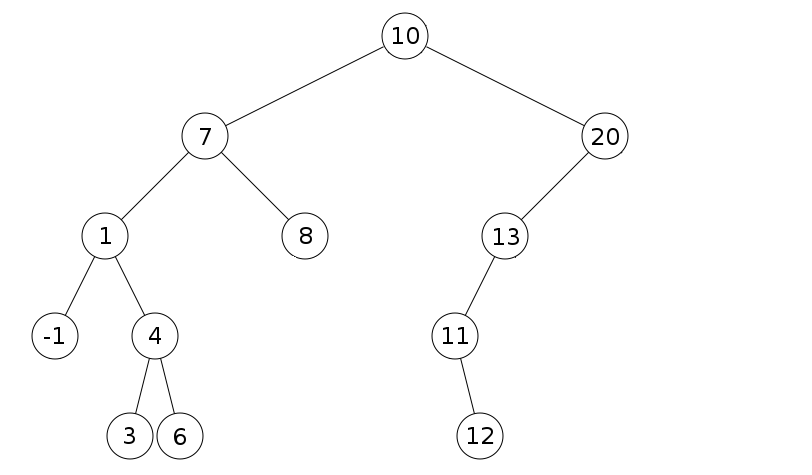
\includegraphics[width=15cm]{kuvat/binaaripuu.png}
\caption{Kuvan \ref{yleinenpuu} solmut järjestettynä eräällä mahdollisella tavalla binäärihakupuuhun.}
\label{binaaripuu}
\end{figure}

Binäärihakupuussa solmun etsimisen aikavaativuus on $\mathcal{O}(h)$, missä $h$ on puun korkeus. Esimerkiksi kuvassa \ref{epatasapaino} esitetyssä binäärihakupuussa solmuun 5 kulkeminen edellyttää kaikkien solmujen läpikäyntiä, eli tässä tapauksessa binääripuu ei ole linkitettyä listaa parempi tietorakenne. Mikäli tälläistä tasapainottamatonta binääripuuta käyttäisi tekstiin, jonka sanat ovat aakkosjärjestyksessä (esimerkiksi sanakirjan hakemisto), on puuhun lisäämisen ja sieltä hakemisen aikavaativuus $\mathcal{O}(n)$ missä $n$ on puun solmujen määrä. \cite{cormen}

\begin{figure}
\centering
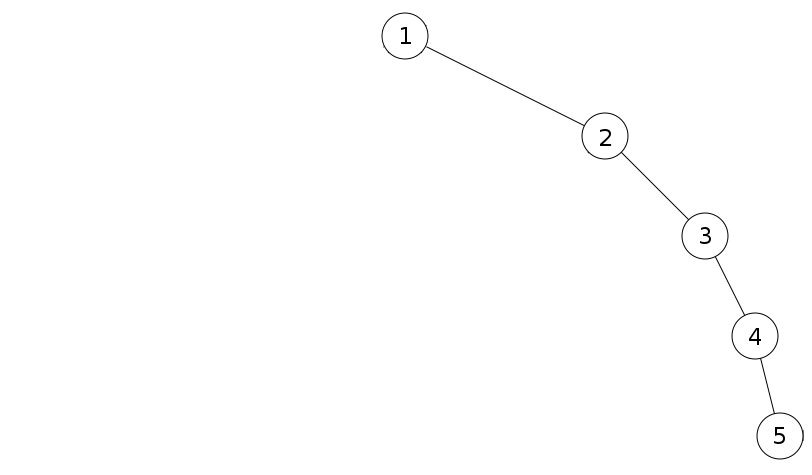
\includegraphics[width=15cm]{kuvat/binaaripuu-epatasapaino.png}
\caption{Hyvin epätasapainoinen binäärihakupuu.}
\label{epatasapaino}
\end{figure}

Siksi binäärihakupuu kannattaakin pyrkiä pitämään jollain tavalla tasapainossa siten, että puun tasapainottamiseen kuluva aika on pienempi kuin siitä saatava hyöty muiden operaatioiden aikavaativuuksissa. Vaihtoehtoisia toteutuksia on useita, muun muassa splay-puut, punamustat puut sekä AVL-puut. Tässä työssä käytetään AVL-puuta. \cite{cormen}

AVL-puun katsotaan olevan tasapainossa jos minkään solmun oikean ja vasemman lapsen korkeuksien ero ei ole suurempi kuin yksi. Mikäli solmun lisääminen tai poistaminen johtaa epätasapainon syntymiseen, se korjataan erilaisilla kierroilla. Kuvassa \ref{avl} on nähtävillä eräs mahdollinen tapa järjestää kuvan \ref{binaaripuu} solmut siten, että puu täyttää AVL-puun tasapainoehdon. \cite{cormen}

\begin{figure}
\centering
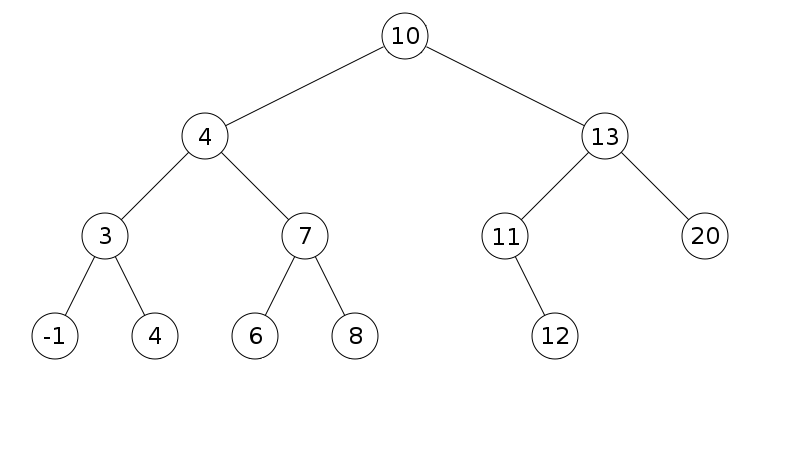
\includegraphics[width=15cm]{kuvat/avlpuu.png}
\caption{AVL-puu}
\label{avl}
\end{figure}


\section{Toteutus}
Sanalaskuria varten toteutin AVL-puun ja tiedostonluvun omina moduuleinaan sekä näitä käyttävän pääohjelman. AVL-puu koostuu solmuista, joista kukin tallentaa korkeintaan 50 merkkiä pitän sanan sekä sanojen esiintymismäärän. Lisäksi solmuun on tallennettu pointteri sen vanhempaan sekä oikeaan ja vasempaan lapseen. Mikäli lasta tai vanhempaa ei ole, on pointteri NULL.

Lisäksi toteutin funktiot tietyn sanan sisältävän solmun etsimiseksi puusta, solmun korkeuden laskemiseksi sekä solmujen lisäämiseksi puuhun. Näitä varten tarvitsin myös puun tasapainottavan funktion sekä sen käyttämät kierrot. Sanalaskurissa solmujen poistaminen on tarpeetonta, joten en toteuttanut sitä puuhun.

Tulosten näyttämiseksi solmulla on myös aliohjelma, joka tulostaa solmuun tallennetun sanan sekä sen lukumäärät. Koko puun tulostamiseksi kirjoitin lisäksi aliohjelman, joka kutsuu edellistä aliohjelmaa kaikille solmusta lähtevän alipuun solmuille, jolloin kaikki puun sanat saadaan tulostettua. Kun solmut tulostetaan sisäjärjestyksessä (ensin vasen lapsi rekursiivisesti, sitten solmu itse, viimeiseksi oikea lapsi rekursiivisesti), tulostuvat solmut aakkosjärjestyksessä.

Tiedostonlukumoduuli lukee avattua tiedostoa rivi (maksimipituus 10~000 merkkiä) kerrallaan ja palauttaa aina funktiota \texttt{lue\_sana()} kutsuttaessa seuraavan sanan tiedostossa. Mikäli rivi loppuu, katsotaan myös sanan loppuvan ja lukeminen aloitetaan seuraavan sanan kohdalla seuraavalta riviltä. Sanoiksi katsotaan yhtenäiset korkeintaan 50 merkin mittaiset merkkijonot, jotka voivat sisältää isoja tai pieniä kirjaimia a-z, numeroita 0-9 ja väliviivoja (-). Kaikkien muiden merkkien katsotaan olevan sanaerottimia eikä niitä käsitellä mitenkään. Ennen sanan palauttamista sen isot kirjaimet muutetaan pieniksi. Mikäli tiedosto on tyhjä tai luettu loppuun, \texttt{lue\_sana()} palauttaa tyhjän merkkijonon.

Luettavan tiedoston voi asettaa tai sitä voi vaihtaa \texttt{avaa(pituus, tiedostonimi)}-\-funktiolla, joka sulkee vanhan tiedoston mikäli sellainen on auki ja avaa sen jälkeen uuden tiedoston käyttäen polkuna annettua tiedostonimeä. Funktio palauttaa true mikäli tiedoston avaaminen onnistuu ja false mikäli ei onnistu. Jälkimmäisessä tapauksessa ohjelma tulostaa myös virheviestin, joka kertoo, mikä iostatin arvo oli. Samalla funktiolla voi myös siirtää lukukohdan takaisin tiedoston alkuun avaamalla jo auki olevan tiedoston uudelleen.

Pääohjelma sanalaskuri ottaa komentoriviargumenttina polun tutkittavaan tiedostoon ja yrittää avata kyseisen tiedoston. Mikäli argumentteja ei ole, ohjelma tulostaa virheviestin ja suoritus lopetataan. Myös tiedoston avaamisen epäonnistuessa ohjelman suoritus pysäytetään. Onnistuneen tiedoston avaamisen jälkeen luetaan tiedoston ensimmäinen sana AVL-puun juureksi. Mikäli tämä sana on tyhjä, tiedetään tiedoston olevan tyhjä. Jos taas sana ei ole tyhjä, luetaan uusia sanoja ja lisätään niitä puuhun, kunnes \texttt{lue\_sana()}-funktio palauttaa tyhjän sanan, minkä jälkeen kutsutaan AVL-puun aliohjelmaa, joka tulostaa puun.

Ohjelman kääntämiseksi kirjoitin makefilen, jolloin ohjelma voidaan kääntää yksinkertaisesti komennolla \texttt{make} ja tämän jälkeen ajaa muotoa \texttt{./bin/sanalaskuri path/to/file.txt} olevalla komennolla, missä \texttt{path/to/file.txt} on korvattu halutulla tiedostolla.

\section{Tulokset}



\section{Johtopäätökset}
% voishan sen poistonkin tehä
% sanan pituus puussa kovakoodattu

%%%%% Sisältö loppuu, lähdeluettelo %%%%%
\newpage
\bibliographystyle{plain}
\bibliography{lahteet} 
%\appendix
%\newpage
%\section{Käytetty alkuarvotiedosto} \label{alkuarvot}
%\lstinputlisting[basicstyle=\ttfamily]{hr8799.txt}
%\newpage
%\section{Simulointi- ja plottausskripti} \label{skripti}
%\lstinputlisting[basicstyle=\ttfamily,language=bash,showstringspaces=false,breaklines=true]%{skripti.txt}
%\newpage
\end{document}
